% Overview of the proposed execution-aware anytime replanner (vector figure, drawn at print size: 16 cm wide).
% Compile: pdflatex fig_overview.tex  ->  fig_overview.pdf (included by main.tex at \linewidth)
\documentclass[tikz,border=1pt]{standalone}
\usepackage[T1]{fontenc}
\usepackage{newtxtext}
\usepackage[varvw]{newtxmath}
\usetikzlibrary{arrows.meta,calc,positioning,shapes.geometric}
\definecolor{ink}{HTML}{000000}
\definecolor{muted}{HTML}{6B6B6B}
\definecolor{line}{HTML}{3A3A3A}
\definecolor{blue}{HTML}{1F6FC5}
\definecolor{lblue}{HTML}{EDF3FB}
\definecolor{orange}{HTML}{D9622B}
\definecolor{lorange}{HTML}{FCEBDD}
\definecolor{green}{HTML}{178A5E}
\definecolor{lgreen}{HTML}{E1F3EA}
\definecolor{purple}{HTML}{6A4BB5}
\definecolor{lpurple}{HTML}{ECE7F8}
\definecolor{red}{HTML}{C62828}
\definecolor{lgrey}{HTML}{F3F3F1}
\definecolor{sand}{HTML}{F8F3E8}
\tikzset{
  drone/.pic={
    \draw[line width=0.7pt, #1] (-0.17,-0.17) -- (0.17,0.17) (-0.17,0.17) -- (0.17,-0.17);
    \foreach \x/\y in {-0.17/-0.17, 0.17/0.17, -0.17/0.17, 0.17/-0.17}
      \draw[line width=0.6pt, #1, fill=white] (\x,\y) circle (0.085);
    \fill[#1] (0,0) circle (0.06);
  },
  drone/.default=ink,
  task/.style={circle, draw=ink, fill=#1, line width=0.45pt, inner sep=0pt, minimum size=5.5pt},
  task/.default=white,
  S/.style={font=\fontsize{8.4}{9.8}\selectfont, text=ink},
  H/.style={font=\fontsize{9.8}{11}\selectfont\bfseries, text=ink},
  box/.style={draw=line, line width=0.6pt, rounded corners=2.5pt, fill=#1, align=flush center, inner sep=3.2pt,
              font=\fontsize{8.6}{10.2}\selectfont, text=ink},
  box/.default=white,
  arr/.style={-{Stealth[length=5pt,width=4pt]}, line width=0.8pt, draw=ink},
  darr/.style={-{Stealth[length=5pt,width=4pt]}, line width=0.8pt, draw=ink, dash pattern=on 3pt off 2pt},
  panel/.style={draw=line, line width=0.7pt, rounded corners=4pt},
}
\begin{document}
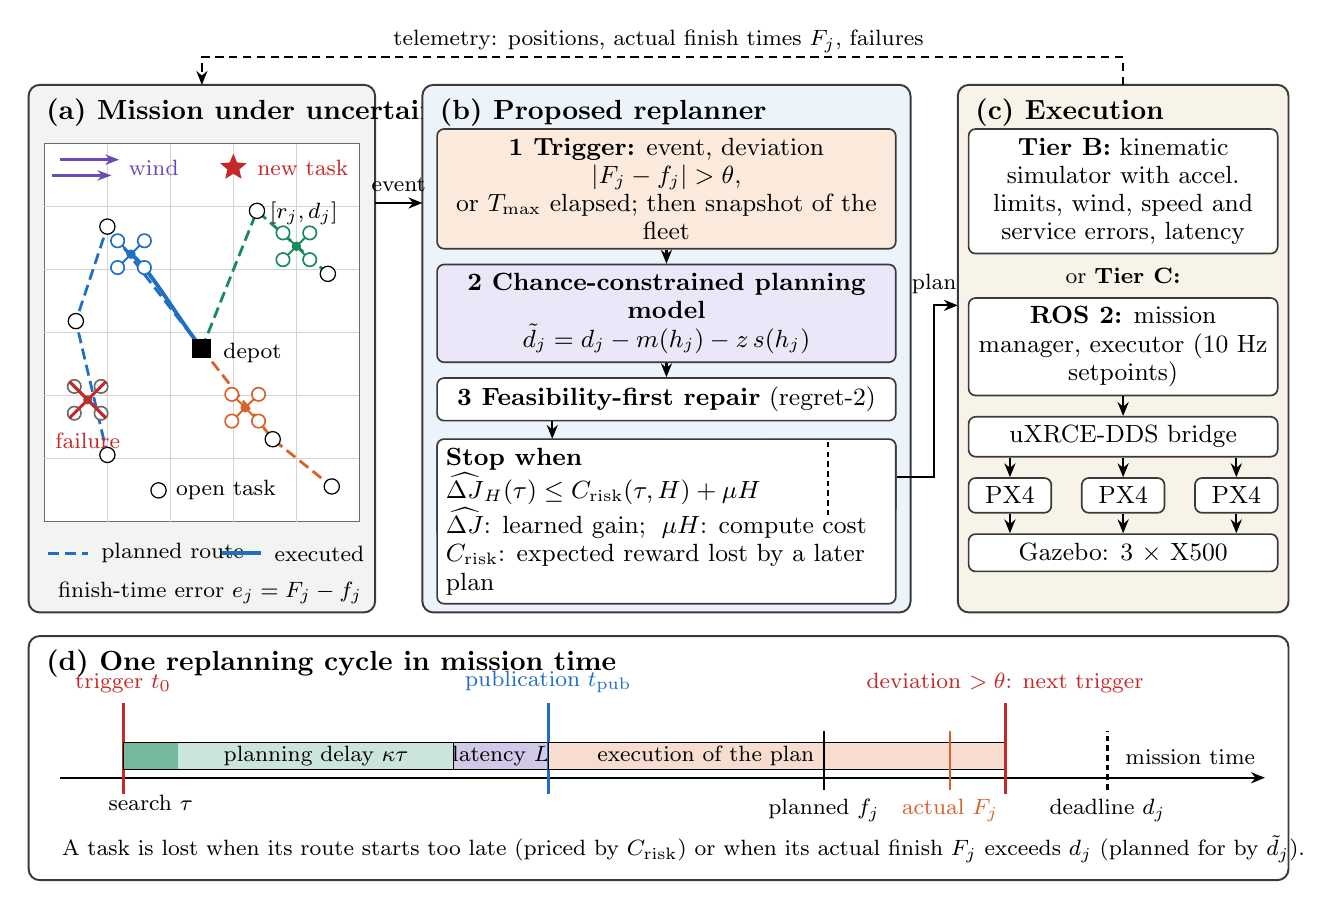
\begin{tikzpicture}
% =================================================================== (a) mission under uncertainty
\fill[lgrey, rounded corners=4pt] (0,3.4) rectangle (4.4,10.1);
\draw[panel] (0,3.4) rectangle (4.4,10.1);
\node[H, anchor=north west] at (0.1,10.05) {(a) Mission under uncertainty};
\fill[white] (0.2,4.55) rectangle (4.2,9.35);
\draw[muted, line width=0.4pt] (0.2,4.55) rectangle (4.2,9.35);
\foreach \x in {1.0,1.8,2.6,3.4} \draw[muted!30, line width=0.3pt] (\x,4.55) -- (\x,9.35);
\foreach \y in {5.35,6.15,6.95,7.75,8.55} \draw[muted!30, line width=0.3pt] (0.2,\y) -- (4.2,\y);
\coordinate (D) at (2.2,6.75);
% planned routes (dashed) and the executed path of the blue UAV (solid, deviating)
\draw[blue, line width=1.0pt, dash pattern=on 4pt off 2pt] (D) -- (1.0,8.3) -- (0.6,7.1) -- (1.0,5.4);
\draw[green, line width=1.0pt, dash pattern=on 4pt off 2pt] (D) -- (2.9,8.5) -- (3.8,7.7);
\draw[orange, line width=1.0pt, dash pattern=on 4pt off 2pt] (D) -- (3.1,5.6) -- (3.85,5.0);
\draw[blue, line width=1.4pt] (D) .. controls (1.85,7.2) and (1.55,7.75) .. (1.3,7.95);
\foreach \p in {(1.0,8.3),(0.6,7.1),(1.0,5.4),(2.9,8.5),(3.8,7.7),(3.1,5.6),(3.85,5.0)} \node[task] at \p {};
\node[S, anchor=west, inner sep=1pt] at (3.02,8.47) {$[r_j, d_j]$};
\node[task] at (1.65,4.95) {};
\node[S, anchor=west] at (1.75,4.95) {open task};
\fill[ink] ($(D)+(-0.12,-0.12)$) rectangle ($(D)+(0.12,0.12)$);
\node[S, anchor=west] at ($(D)+(0.15,-0.05)$) {depot};
\pic at (1.3,7.95) {drone=blue};
\pic at (3.4,8.05) {drone=green};
\pic at (2.75,6.0) {drone=orange};
% events and disturbances
\node[star, star points=5, star point ratio=2.2, fill=red, inner sep=0pt, minimum size=10pt] at (2.6,9.05) {};
\node[S, anchor=west, text=red] at (2.78,9.05) {new task};
\pic at (0.75,6.1) {drone=muted};
\draw[red, line width=1.1pt] (0.52,5.87) -- (0.98,6.33) (0.52,6.33) -- (0.98,5.87);
\node[S, anchor=north, text=red] at (0.75,5.8) {failure};
\draw[-{Stealth[length=5pt]}, line width=1.0pt, purple] (0.4,9.15) -- (1.15,9.15);
\draw[-{Stealth[length=5pt]}, line width=1.0pt, purple] (0.3,8.95) -- (1.05,8.95);
\node[S, text=purple, anchor=west] at (1.15,9.05) {wind};
% legend
\draw[blue, line width=1.0pt, dash pattern=on 4pt off 2pt] (0.25,4.15) -- (0.75,4.15);
\node[S, anchor=west] at (0.8,4.15) {planned route};
\draw[blue, line width=1.4pt] (2.45,4.15) -- (2.95,4.15);
\node[S, anchor=west] at (3.0,4.15) {executed};
\node[S, anchor=west] at (0.25,3.65) {finish-time error $e_j = F_j - f_j$};

% =================================================================== (b) proposed replanner
\begin{scope}[shift={(5.0,0)}]
\fill[lblue, rounded corners=4pt] (0,3.4) rectangle (6.2,10.1);
\draw[panel] (0,3.4) rectangle (6.2,10.1);
\node[H, anchor=north west] at (0.1,10.05) {(b) Proposed replanner};
\tikzset{wide/.style={box=#1, text width=5.6cm}}
\node[wide=lorange, anchor=north] (trig) at (3.1,9.55)
  {\textbf{1 Trigger:} event, deviation $|F_j - f_j| > \theta$,\\or $T_{\max}$ elapsed; then snapshot of the fleet};
\node[wide=lpurple, below=0.18cm of trig] (cc)
  {\textbf{2 Chance-constrained planning model}\\$\tilde d_j = d_j - m(h_j) - z\,s(h_j)$};
\node[wide=white, below=0.18cm of cc] (ffr) {\textbf{3 Feasibility-first repair} (regret-2)};
\node[box=lgreen, text width=2.7cm, below=0.22cm of ffr.south west, anchor=north west] (alns)
  {\textbf{4 Anytime ALNS}\\destroy / repair};
\node[box=lgreen, text width=1.5cm, minimum height=0.95cm, anchor=north east] (stop) at (ffr.south east |- alns.north)
  {\textbf{5 Stop?}};
\draw[arr] (trig) -- (cc);
\draw[arr] (cc) -- (ffr);
\draw[arr] (ffr.south -| alns.north) -- (alns.north);
\draw[arr] ([yshift=-6pt]alns.east) -- ([yshift=-6pt]stop.west);
\draw[arr] ([yshift=6pt]stop.west) -- node[S, above] {no} ([yshift=6pt]alns.east);
\draw[arr] (stop.east) -- (6.5,0 |- stop.east) |- (6.8,7.3);
\node[S, anchor=south] at (6.5,7.32) {plan};
\node[box=white, text width=5.6cm, align=flush left, anchor=south] (rule) at (3.1,3.5)
  {\textbf{Stop when} $\widehat{\Delta J}_{H}(\tau) \le C_{\mathrm{risk}}(\tau,H) + \mu H$\\
   $\widehat{\Delta J}$: learned gain;\; $\mu H$: compute cost\\
   $C_{\mathrm{risk}}$: expected reward lost by a later plan};
\draw[line width=0.7pt, dash pattern=on 2pt off 1.5pt] (stop.south) -- (stop.south |- rule.north);
\end{scope}

% =================================================================== (c) execution
\begin{scope}[shift={(11.8,0)}]
\fill[sand, rounded corners=4pt] (0,3.4) rectangle (4.2,10.1);
\draw[panel] (0,3.4) rectangle (4.2,10.1);
\node[H, anchor=north west] at (0.1,10.05) {(c) Execution};
\node[box=white, text width=3.7cm, anchor=north] (b) at (2.1,9.55)
  {\textbf{Tier B:} kinematic simulator with accel.\ limits, wind, speed and service errors, latency};
\node[S, below=0.05cm of b] (or) {or \textbf{Tier C:}};
\node[box=white, text width=3.7cm, below=0.05cm of or] (ros) {\textbf{ROS 2:} mission manager, executor (10 Hz setpoints)};
\node[box=white, text width=3.7cm, below=0.25cm of ros] (dds) {uXRCE-DDS bridge};
\node[box=white, minimum width=1.05cm, below=0.25cm of dds.south west, anchor=north west] (p1) {PX4};
\node[box=white, minimum width=1.05cm, below=0.25cm of dds.south, anchor=north] (p2) {PX4};
\node[box=white, minimum width=1.05cm, below=0.25cm of dds.south east, anchor=north east] (p3) {PX4};
\node[box=white, text width=3.7cm, below=0.25cm of p2] (gz) {Gazebo: 3 $\times$ X500};
\draw[arr] (ros) -- (dds);
\foreach \p in {p1,p2,p3} { \draw[arr] (dds.south -| \p.north) -- (\p.north); \draw[arr] (\p.south) -- (\p.south |- gz.north); }
\end{scope}

% =================================================================== links between panels
\draw[arr] (4.4,8.6) -- (5.0,8.6);
\node[S, anchor=south] at (4.7,8.62) {event};
\draw[darr] (13.9,10.1) -- (13.9,10.45) -- (2.2,10.45) -- (2.2,10.1);
\node[S, anchor=south, fill=white, inner sep=1pt] at (8.0,10.47) {telemetry: positions, actual finish times $F_j$, failures};

% =================================================================== (d) timeline of one replanning cycle
\fill[white, rounded corners=4pt] (0,0) rectangle (16.0,3.1);
\draw[panel] (0,0) rectangle (16.0,3.1);
\node[H, anchor=north west] at (0.1,3.05) {(d) One replanning cycle in mission time};
\draw[arr] (0.4,1.3) -- (15.7,1.3);
\node[S, anchor=south east] at (15.7,1.35) {mission time};
\draw[line width=1.1pt, red] (1.2,1.1) -- (1.2,2.25);
\node[S, anchor=south, text=red] at (1.2,2.25) {trigger $t_0$};
\fill[green!60] (1.2,1.4) rectangle (1.9,1.75);
\fill[green!22] (1.9,1.4) rectangle (5.4,1.75);
\draw[line width=0.4pt] (1.2,1.4) rectangle (5.4,1.75);
\node[S] at (3.65,1.575) {planning delay $\kappa\tau$};
\node[S, anchor=north] at (1.55,1.2) {search $\tau$};
\fill[purple!30] (5.4,1.4) rectangle (6.6,1.75);
\draw[line width=0.4pt] (5.4,1.4) rectangle (6.6,1.75);
\node[S] at (6.0,1.575) {latency $L$};
\draw[line width=1.1pt, blue] (6.6,1.1) -- (6.6,2.25);
\node[S, anchor=south, text=blue] at (6.6,2.25) {publication $t_{\mathrm{pub}}$};
\fill[orange!22] (6.6,1.4) rectangle (12.4,1.75);
\draw[line width=0.4pt] (6.6,1.4) rectangle (12.4,1.75);
\node[S] at (8.6,1.575) {execution of the plan};
\draw[line width=0.9pt] (10.1,1.15) -- (10.1,1.9);
\node[S, anchor=north] at (10.1,1.15) {planned $f_j$};
\draw[line width=0.9pt, orange] (11.7,1.15) -- (11.7,1.9);
\node[S, anchor=north, text=orange] at (11.7,1.15) {actual $F_j$};
\draw[line width=1.1pt, red] (12.4,1.1) -- (12.4,2.25);
\node[S, anchor=south, text=red] at (12.4,2.25) {deviation $>\theta$: next trigger};
\draw[line width=0.9pt, dash pattern=on 2pt off 1.5pt] (13.7,1.15) -- (13.7,1.9);
\node[S, anchor=north] at (13.7,1.15) {deadline $d_j$};
\node[S, anchor=south west] at (0.3,0.1)
  {A task is lost when its route starts too late (priced by $C_{\mathrm{risk}}$) or when its actual finish $F_j$ exceeds $d_j$ (planned for by $\tilde d_j$).};
\end{tikzpicture}
\end{document}
